% ==============================================================================
% SEÇÃO 4: INTEGRAÇÃO COMPLEMENTAR COM PYTHON (PADRÃO CACHE-ASIDE)
% ==============================================================================
\changecolours{ScoutBlue}
\section{Integração Complementar com Python: Cache-Aside}

\begin{frame}{O Padrão Arquitetural Cache-Aside (Lazy Loading)}
  \centering
  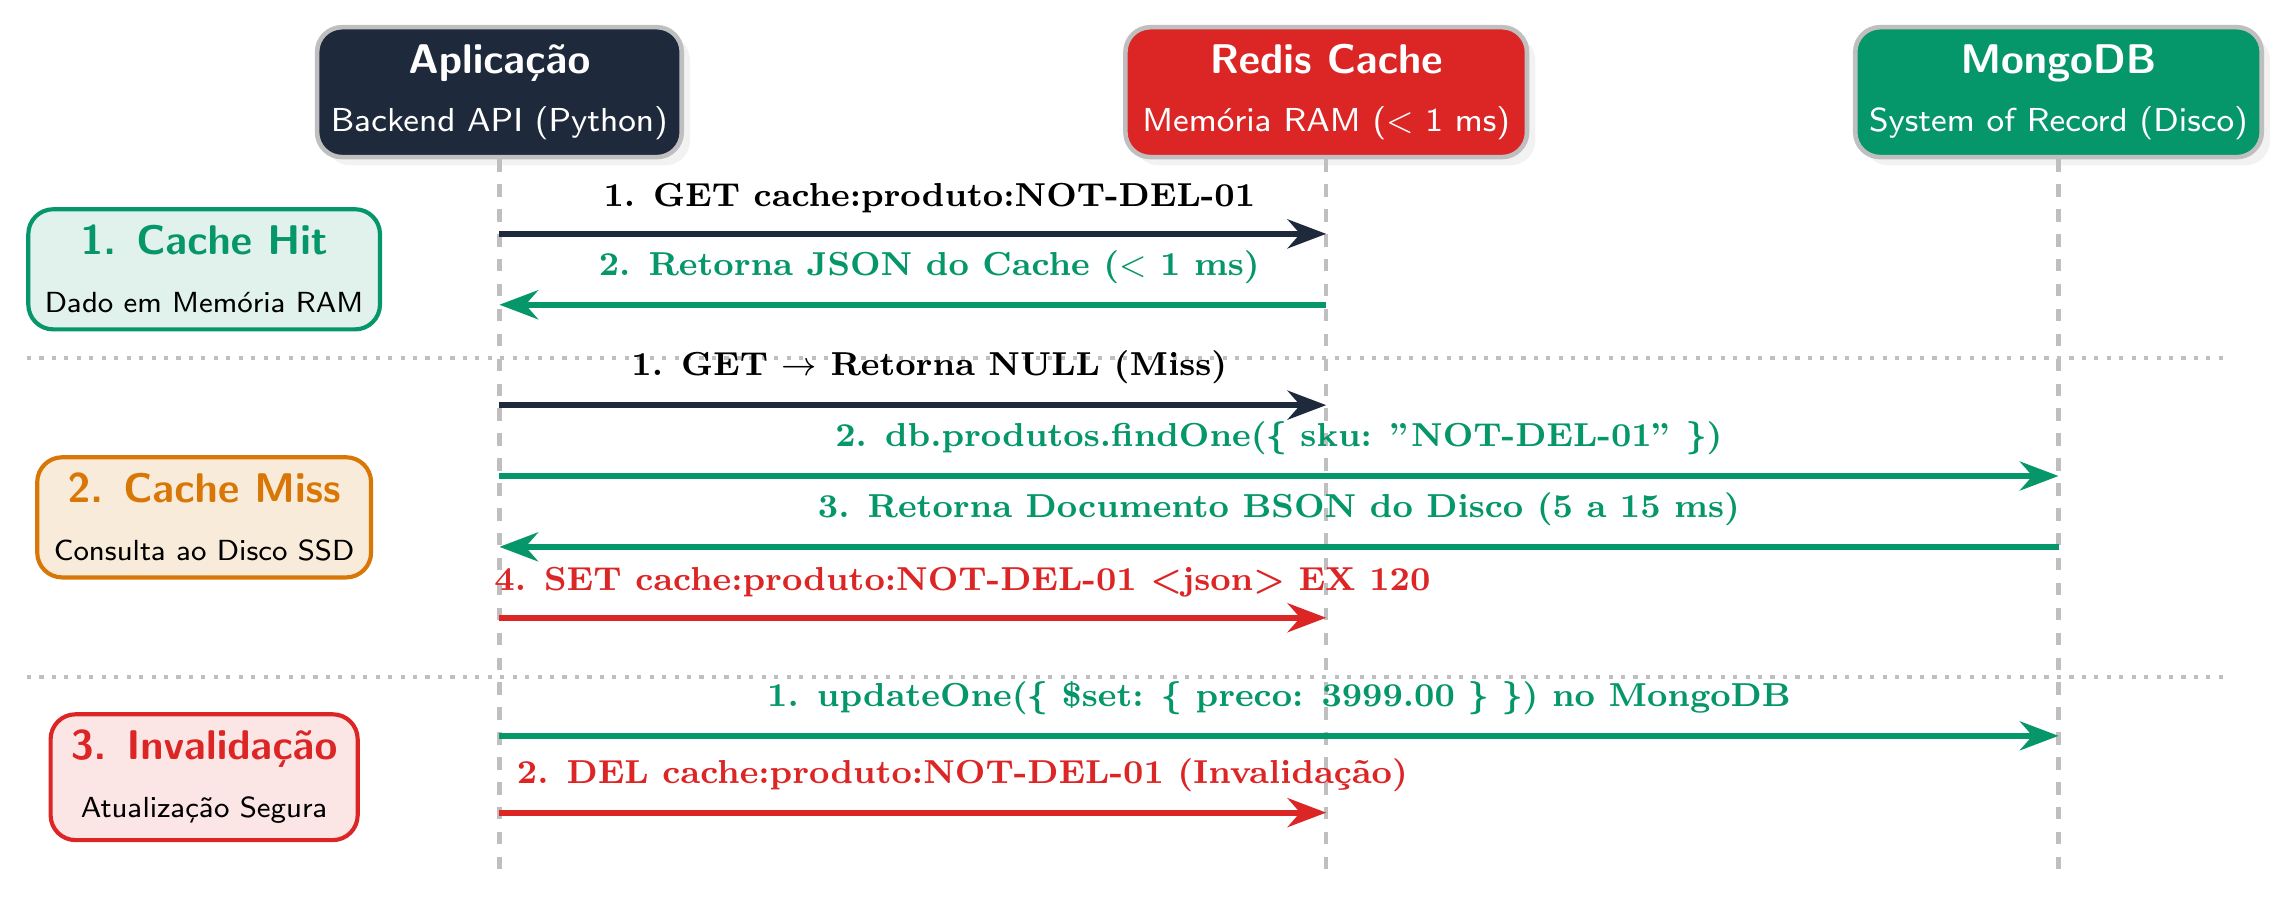
\includegraphics[width=0.98\textwidth,height=0.82\textheight,keepaspectratio]{figuras/fig_cache_aside_pattern.png}
\end{frame}

\begin{frame}[fragile]{Cache-Aside em Python: Verificação e Cache Hit}
  \textbf{Fluxo de Consulta em Memória RAM (Sub-milissegundo):}
\begin{lstlisting}[basicstyle=\ttfamily\scriptsize]
def obter_produto(sku: str, mongo_col, redis_cli, ttl=120):
    cache_key = f"cache:produto:{sku}"
    
    # 1. Tenta recuperar da memoria RAM (Redis)
    dado_cache = redis_cli.get(cache_key)
    if dado_cache:
        return json.loads(dado_cache), "CACHE_HIT"
\end{lstlisting}
  {\footnotesize
  \begin{itemize}
    \item \textbf{Cache Hit:} Resposta imediata da RAM ($< 1$ ms) sem sobrecarregar o MongoDB.
  \end{itemize}
  }
\end{frame}

\begin{frame}[fragile]{Cache-Aside em Python: Cache Miss e População}
  \textbf{Fallback no MongoDB e Armazenamento com TTL:}
\begin{lstlisting}[basicstyle=\ttfamily\scriptsize]
    # 2. CACHE MISS: Busca na fonte da verdade (MongoDB)
    produto_db = mongo_col.find_one({"sku": sku}, {"_id": 0})
    if not produto_db:
        return None, "NOT_FOUND"
        
    # 3. Popula o cache no Redis com tempo de vida definido (TTL)
    redis_cli.set(cache_key, json.dumps(produto_db), ex=ttl)
    return produto_db, "CACHE_MISS"
\end{lstlisting}
  {\footnotesize
  \begin{itemize}
    \item \textbf{Lazy Loading Idempotente:} O cache só é abastecido sob demanda, otimizando a memória RAM.
  \end{itemize}
  }
\end{frame}

\begin{frame}[fragile]{Invalidação de Cache e Prevenção de Dados Obsoletos}
  \begin{columns}[T]
    \begin{column}{0.52\textwidth}
      \textbf{Atualização com Invalidação}
\begin{lstlisting}[basicstyle=\ttfamily\scriptsize]
def atualizar_preco(sku, preco, col, r):
  # 1. Atualiza MongoDB
  col.update_one(
    {"sku": sku},
    {"$set": {"preco": preco}}
  )
  # 2. Invalida no Redis
  r.delete(f"cache:prod:{sku}")
\end{lstlisting}
    \end{column}

    \begin{column}{0.46\textwidth}
      \begin{block}{O Risco de Stale Read}
        {\footnotesize
        Sem invalidação ativa imediata:
        \begin{itemize}
          \item Usuários visualizam dados defasados até o TTL expirar.
          \item O comando \texttt{DEL} força o próximo acesso a buscar o valor atualizado na fonte oficial.
        \end{itemize}
        }
      \end{block}
    \end{column}
  \end{columns}
\end{frame}

\begin{frame}{Resultados Empíricos: Benchmarking de Latência}
  \centering
  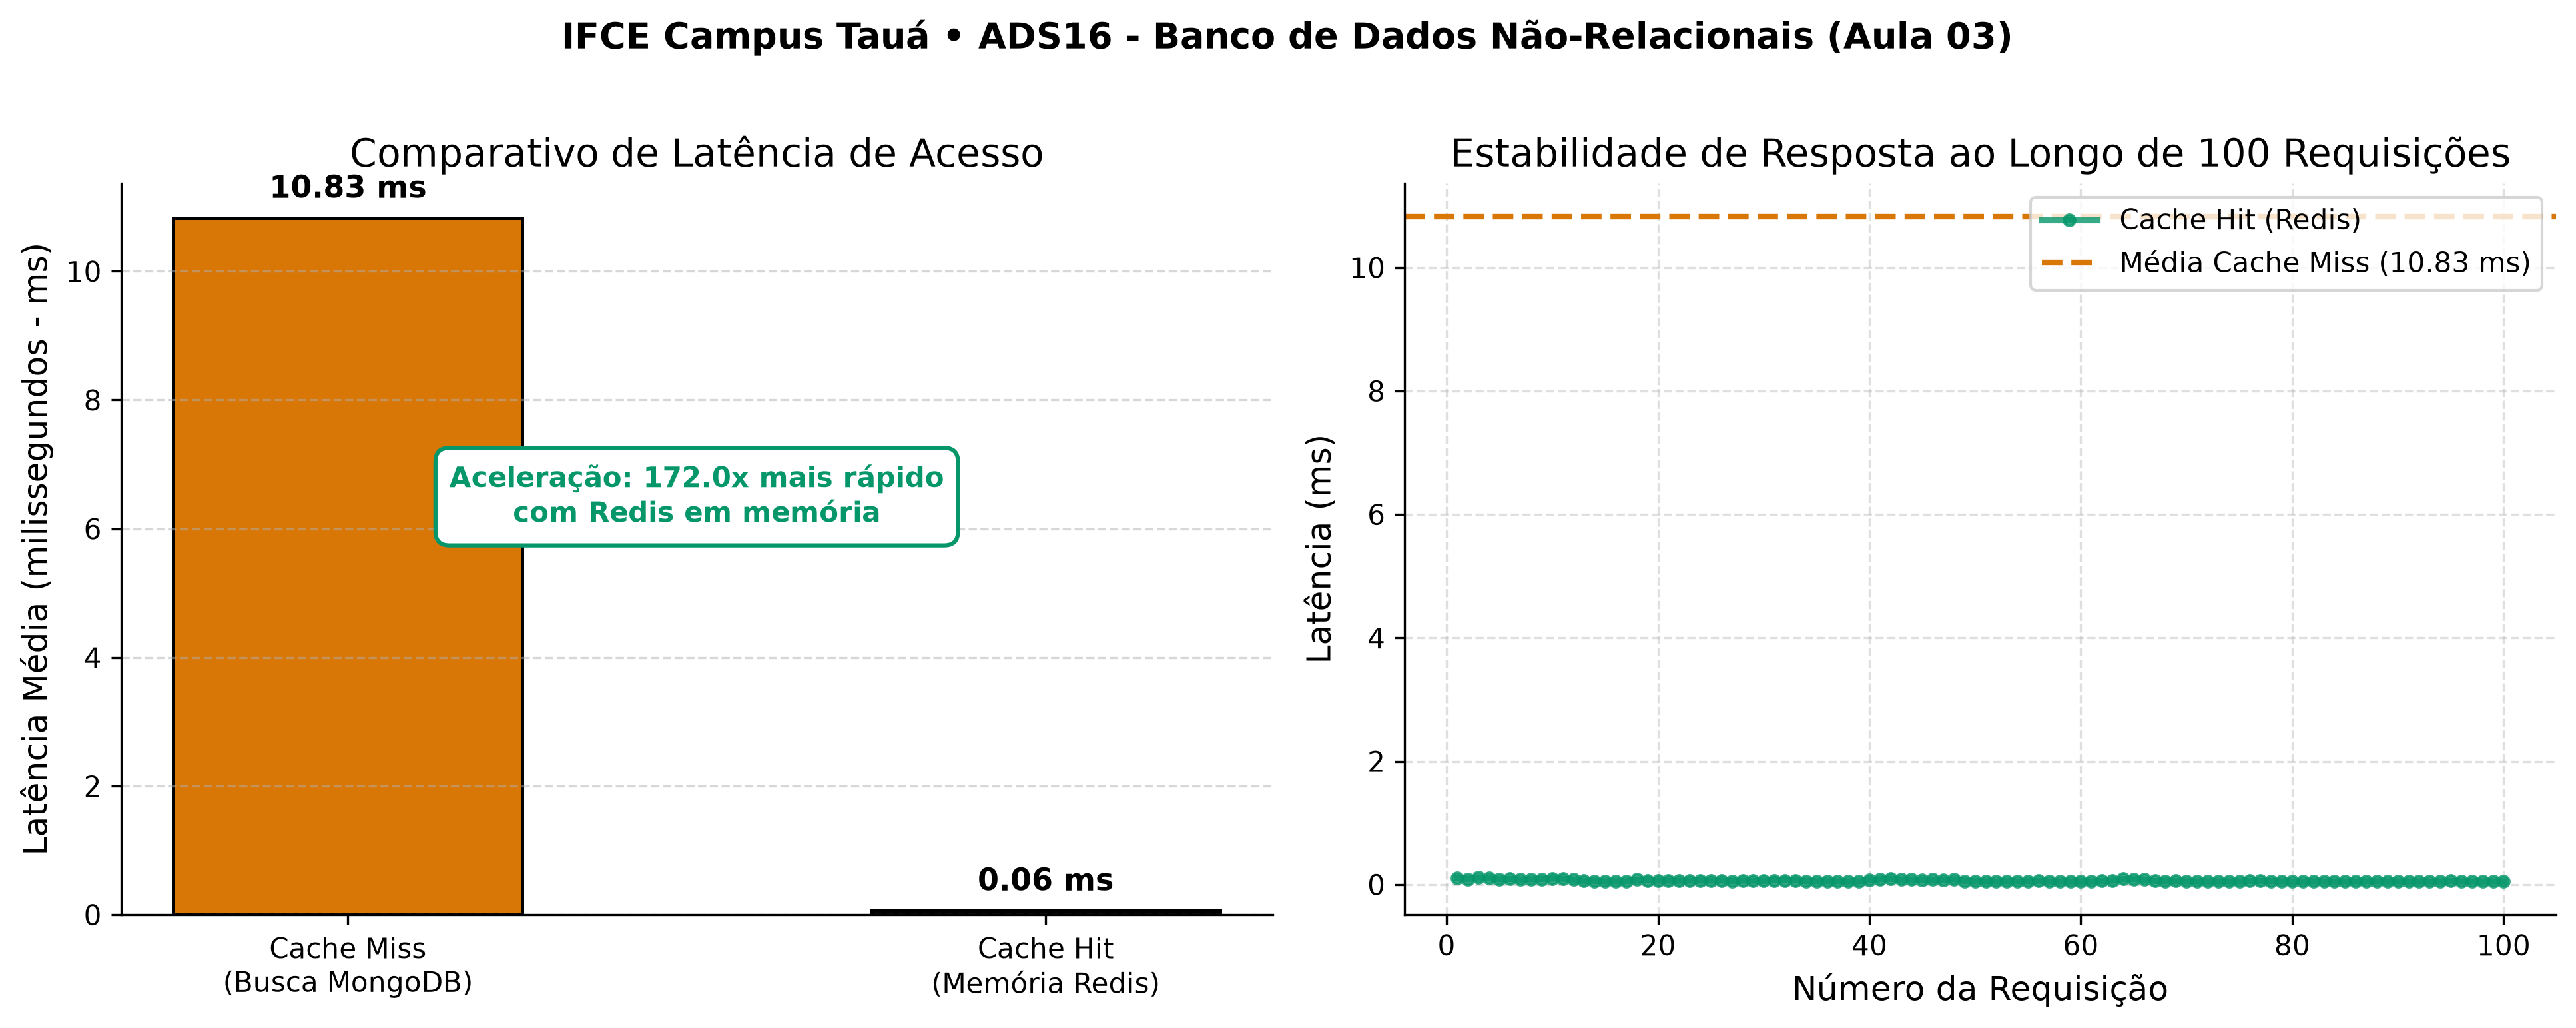
\includegraphics[width=0.98\textwidth,height=0.82\textheight,keepaspectratio]{figuras/grafico_latencia_cache.png}
\end{frame}
